\section{Conceptual design options} \label{ch:options}
This chapter will discuss the five design concepts that will be considered in this report. First in section \ref{sec:consel} the selection of concepts based on the shape, mission duration and controls system design option trees is made. For the six configurations of the \gls{br} one is disregarded as it has no additional advantages over the other concepts. In section \ref{sec:conf} the five selected configurations are sketched and described. A simple load analysis is given in the form of \gls{fbd} to gain insight in the functioning of each of the concepts. The following five designs are consequently used for analysis in the relevant chapters of this report. Finally the control systems corresponding to the each of the shape configurations are discussed in chapter \ref{sec:ccs}. A full definition of the control system is not yet given but is rather further detailed in the \gls{fr}. Only the feasibility and risk associated with the various combinations will be assessed.



\subsection{Concept selection} \label{sec:consel}
 From the \acrfull{br} three \glspl{dot} were obtained for the design of the \gls{hiad}. In these design concepts shape, mission duration and control system were considered. This yielded a set of all the individual design options. These options are shown in Figures \ref{fig:dotshape} to \ref{fig:dotduration}. From these \glspl{dot} a feasible set of design options can be obtained. In Figure  \ref{fig:dotshape} six concept configurations deemed feasible are distinguished. These can be combined with three possible control systems from Figure  \ref{fig:dotcontrol}. The mission duration varies for all concepts and is therefore considered separately for every design concept. The mission duration appears in the form of a trade-off criterion discussed further in chapter \ref{ch:tradeoff} discussing the trade-off criteria.

\begin{figure}[H]
%\centering
\hspace{-23mm}
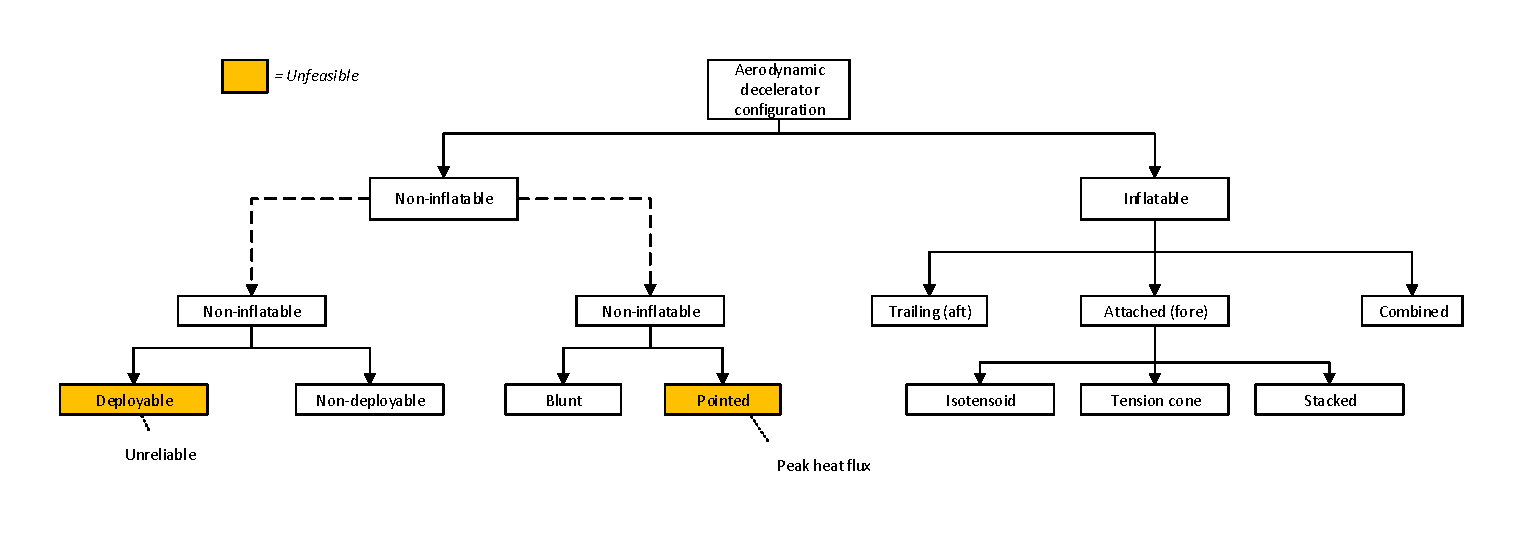
\includegraphics[width = 1.25\textwidth]{Figure/DOT_configuration.pdf}
\vspace{-5mm}
\caption{\acrfull{dot} for entry vehicle configurations}
\label{fig:dotshape}
\end{figure}

\begin{figure}[H]
\centering
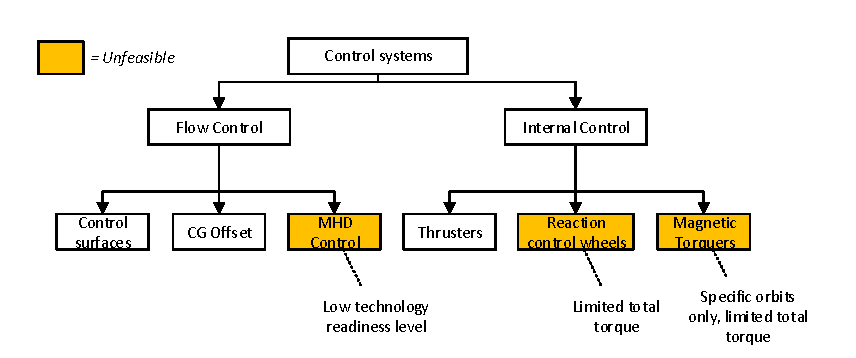
\includegraphics[width = 0.93\textwidth]{Figure/DOT_control.pdf}
\vspace{-5mm}
\caption{\acrfull{dot} for control systems}
\label{fig:dotcontrol}
\end{figure}

\begin{figure}[H]
\centering
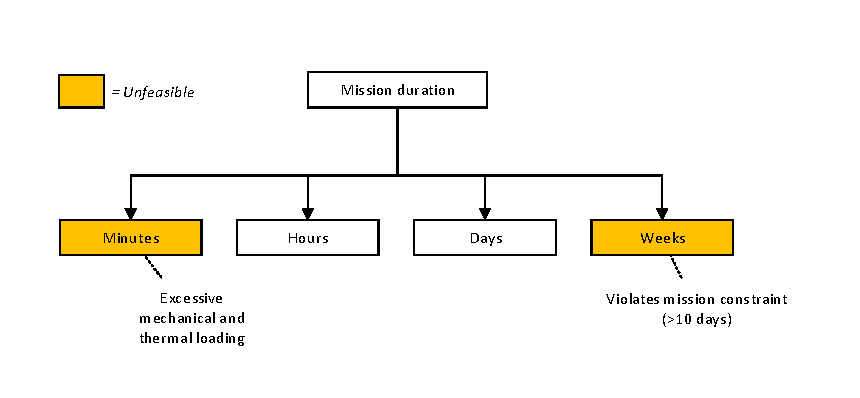
\includegraphics[width = 1.0\textwidth]{Figure/DOT_missionduration.pdf}
\vspace{-5mm}
\caption{\acrfull{dot} for mission duration}
\label{fig:dotduration}
\end{figure}

From the eighteen options yielded by combining the six feasible shapes and three feasible control systems shown in Figures \ref{fig:dotshape} and \ref{fig:dotcontrol} some may be disregarded immediately since they cannot practically be combined. For obvious reasons it is crucial that each concept configuration features at least one deemed feasible control system. From this point onward the concept shape will be considered leading. 

The control systems from Figure  \ref{fig:dotcontrol} are considered separately for each of these shapes. Due to infeasibility of exotic control concepts such as the, for now, deemed infeasible \gls{mhd} the control system can be integrated with each structure. This can be done since the control systems themselves do no longer require strict geometric properties as would be required by for example \gls{mhd} control. The control systems are only used to check whether feasible options exist.

Table \ref{tab:designconcepts} shows the design options that will be considered within this report. The check-marked control systems are further investigated for their feasibility and performance within section \ref{sec:ccs}. The configurations are further detailed in section \ref{sec:conf}. It must be noted that the control configurations of Table \ref{tab:designconcepts} feature the primary control mechanism. These may always be supplemented later on in the design process, after the trade-off, if additional control systems increase the overall systems performance. 

\begin{table}[H]
	\caption{Generation of design concepts}
	\label{tab:designconcepts}
	\centering
		\begin{tabular}{|p{0.3\textwidth}|p{0.14\textwidth}|p{0.14\textwidth}|p{0.14\textwidth}|} \hline 
			\textbf{Concept} & \textbf{Thrusters}	& \textbf{\gls{cg} offset} &  \textbf{Control surfaces} \\ \hline \hline
			Stacked toroid   & \cmark	& \cmark &  \cmark \\ \hline
			Isotensoid		 & \cmark	& \cmark &  \xmark\\  \hline
			Tension cone	 & \cmark	& \cmark &  \cmark \\ \hline
			Trailing ballute & \xmark	& \xmark &  \cmark \\ \hline
			Combined 		 & \xmark	& \xmark &  \cmark \\ \hline
			Rigid  		   	 & \cmark	& \cmark &  \cmark \\ \hline
		\end{tabular}
\end{table}

From Table \ref{tab:designconcepts} it can be noted that all shape configurations are deemed feasible for at least one control system. To yield a total of five concepts the combined concept is disregarded for the following reasons. It is considered to be too similar to a Trailing concept. A trailing concept will still require a heat shield in front of the payload and can therefore be considered, in some aspects, a combined configuration as well. It is therefore considered that a deployable inflatable at the front will have no additional advantage. A small deployable will have a similar performance as the trailing configuration, but features the additional complexity of the front inflation system. A large frontal inflatable will however place the aft inflatable in its wake making it effectively useless. Removing the aft declarator will however yield a `simple' stacked toroid, isotensoid or tension cone configuration. For these reasons the combined concept will not be considered. 
 
 The infeasible combinations of control systems are further detailed in section \ref{sec:ccs}, together with a general description of control systems. 
 

\subsection{Concept configurations} \label{sec:conf}
In this section the global configuration of each of the final five shapes is considered. They are sketched \footnote{\label{fn:irene} Courtesy of Irene Heemskerk.} and described shortly in the sections below. Moreover a simple \gls{fbd} is provided to gain insight in, where applicable, the structural principle of each of the concepts and identify where the highest loads occur within the structure. 

\paragraph{Stacked toroid}

Figures \ref{fig:conc_stacked} and \ref{fig:fbd_stacked} show the stacked toroid concept. A stacked toroid configuration features multiple inflatables which are stacked together to form the aeroshell. These inflatables are consequently covered with a thermal protection layer. In this design the payload is placed aft of the aeroshell.


\begin{figure}[H]
\centering
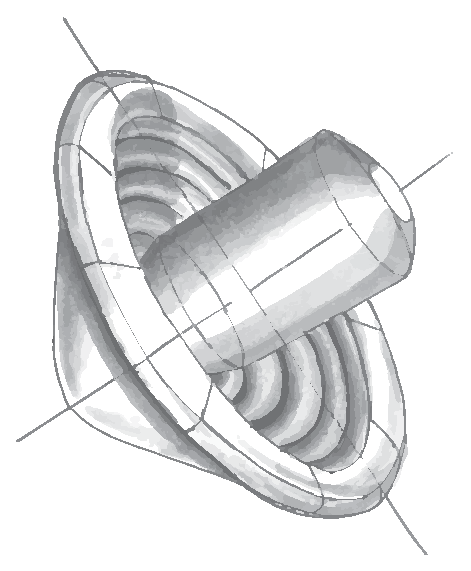
\includegraphics[width = 0.45\textwidth]{Figure/stacked_toroid.eps}
\caption[An impression of a stacked toroid configuration.]{An impression of a stacked toroid configuration\textsuperscript{\ref{fn:irene}}}
\label{fig:conc_stacked}
\end{figure}

\begin{figure}[H]
\centering
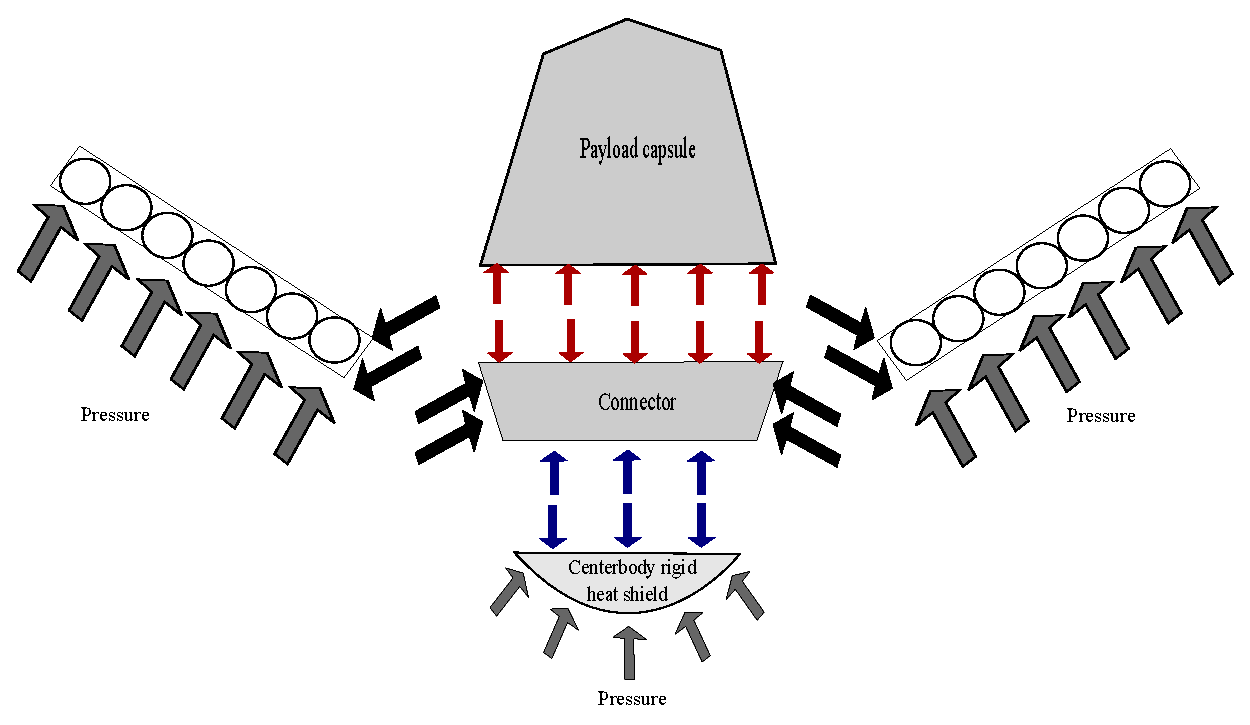
\includegraphics[width = 0.62\textwidth]{Figure/FBD_stacked.eps}
\caption{A \gls{fbd} of the stacked toroid configuration}
\label{fig:fbd_stacked}
\end{figure}

It may be observed from Figure  \ref{fig:fbd_stacked} that the inflatable parts are in compression and incur most of the aerodynamic loads. Buckling is therefore a structural consideration to be taken into account. Internal pressure counters the aerodynamic pressure working on the toroids. The aerodynamic loads, denoted by the black arrows are transferred to the rigid centerbody by a set of center rings, where loads are highly concentrated. Moreover, loads are distributed within the centerbody, consisting of payload capsule, connector and rigid heat shied, as denoted by the red and blue arrows.


\paragraph{Isotensoid}

An isotensoid configuration as displayed in Figures \ref{fig:conc_iso} and \ref{fig:fbd_iso} features a single inflatable. This inflatable covers the whole of the payload. This inflatable is relatively large and is typically inflated using ram-air \cite{Smith2011}. 

\begin{figure}[H]
\centering
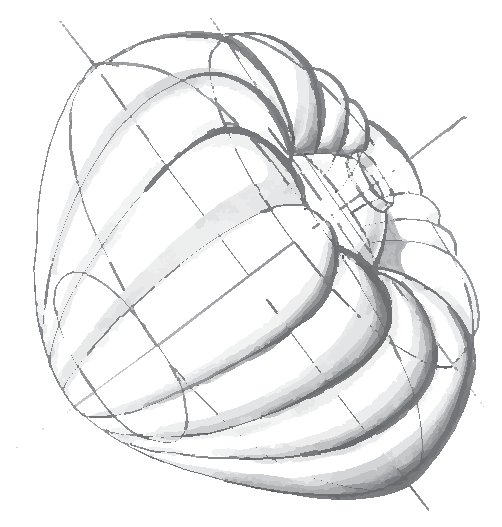
\includegraphics[width = 0.45\textwidth]{Figure/isotensoid.eps}

\caption[An impression of an isotensoid configuration]{An impression of an isotensoid configuration\textsuperscript{\ref{fn:irene}}}

\label{fig:conc_iso}
\end{figure}

\begin{figure}[H]
\centering
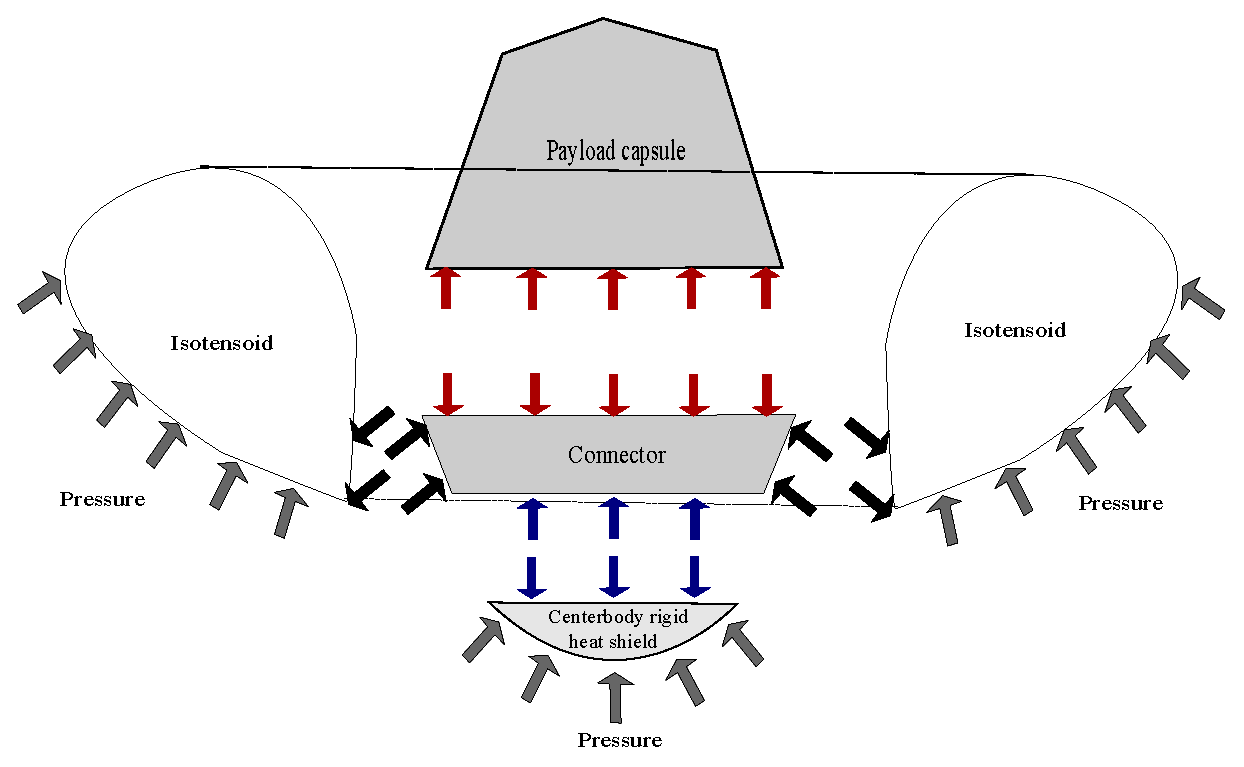
\includegraphics[width = 0.55\textwidth]{Figure/FBD_isotensoid.eps}
\caption{A \gls{fbd} of the isotensoid configuration}
\label{fig:fbd_iso}
\end{figure}

From Figure  \ref{fig:fbd_iso} it may be observed that the inflatable bladder is in compression by aerodynamic pressure. Internal pressure, built up by ram-air inflation, brings the structure in equilibrium and thereby preserves its shape. Loads are transferred to the centerbody by a number of center rings, similar to the stacked toroid configuration.

\paragraph{Tension cone}

A tension cone, as shown in Figures  \ref{fig:conc_tension} and \ref{fig:fbd_tension} also consists of a single inflatable. In this case the inflatable is ring shaped, using the ring to provide stiffness to a membrane spanned within. In this configuration the aeroshell is placed in front of the payload, warping around it in some extend.

\begin{figure}[H]
\centering
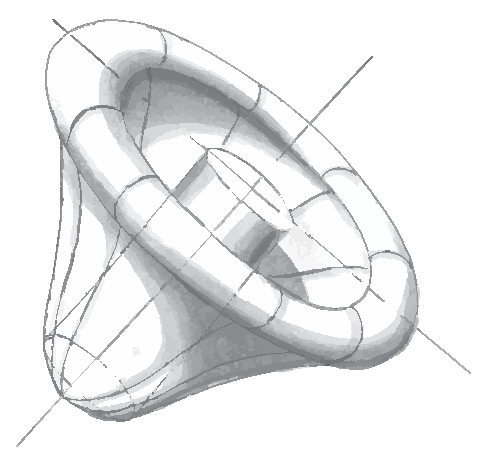
\includegraphics[width = 0.45\textwidth]{Figure/tension_cone.eps}

\caption[An impression of of a tension cone configuration]{An impression of of a tension cone configuration\textsuperscript{\ref{fn:irene}}}

\label{fig:conc_tension}
\end{figure}

\begin{figure}[H]
\centering
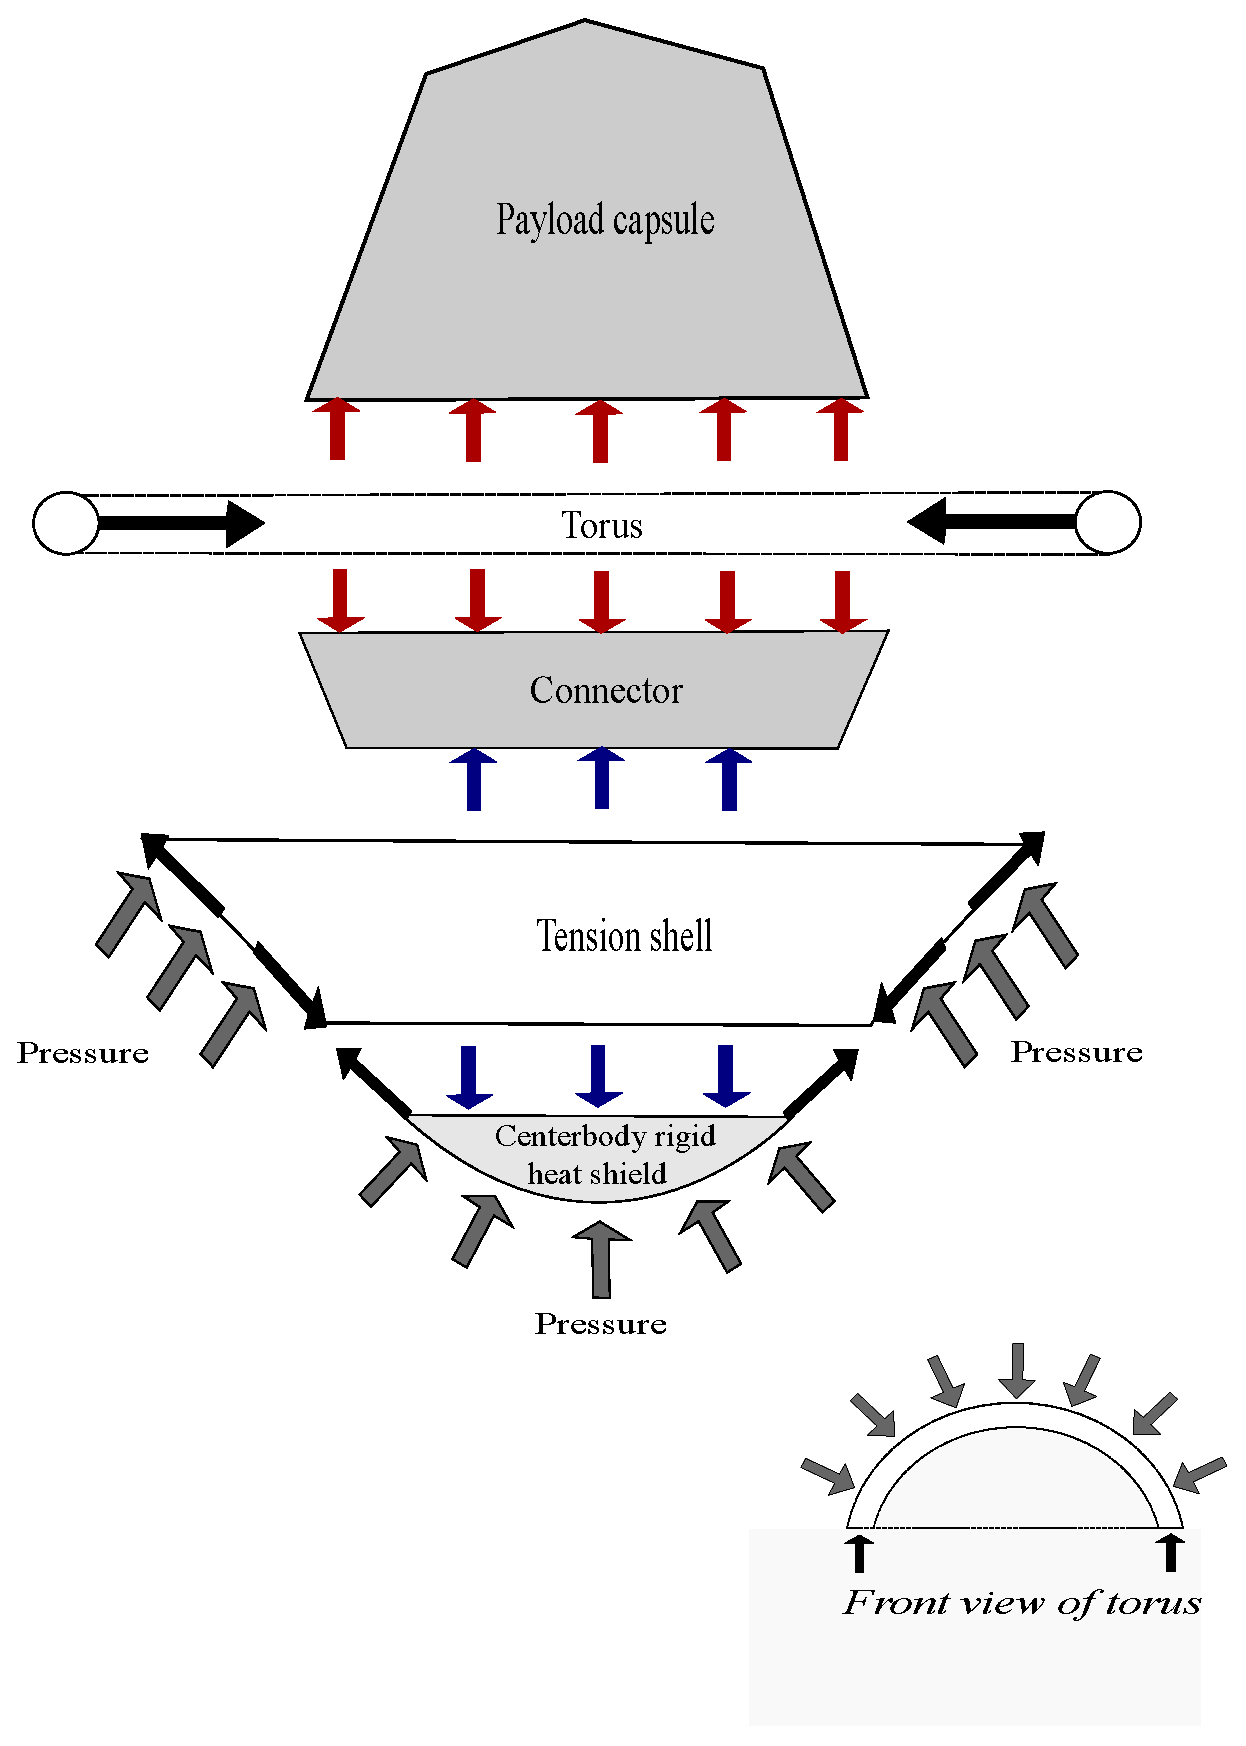
\includegraphics[width = 0.4\textwidth]{Figure/FBD_tensioncone.eps}
\caption{A \gls{fbd} of the tension cone configuration}
\label{fig:fbd_tension}
\end{figure}

The \gls{fbd} in Figure  \ref{fig:fbd_tension} shows that the inflatable torus is in compression. Similar to the other inflatable concepts, this compressive force is counteracted by an internal pressure inflating the torus. The tension shell is in tension (from which it derives its name). 

\paragraph{Trailing}

Figures \ref{fig:conc_trailing} and \ref{fig:fbd_trailing} show a trailing ballute configuration. A trailing configuration consist of two parts. An aft-placed inflatable, typically referred to as the trailing, and a front placed rigid heat shield. Since the inflatable is placed aft the payload is directly exposed to the atmosphere requiring an additional rigid heat shield. The shock waves induced by the front of the payload consequently create a wake aft of the payload. A typical trailing device is therefore ring formed to stay out of this wake. This is also displayed in Figure  \ref{fig:conc_trailing}. This is also the trailing configuration as treated within this report.

\begin{figure}[H]
\centering
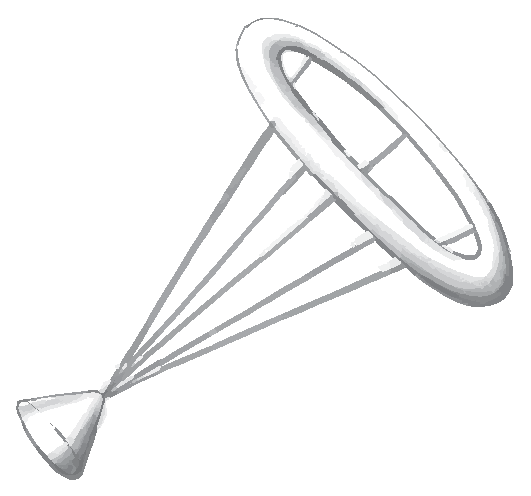
\includegraphics[width = 0.5\textwidth]{Figure/trailing_ballute.eps}

\caption[An impression of a trailing configuration]{An impression of a trailing configuration\textsuperscript{\ref{fn:irene}}}

\label{fig:conc_trailing}
\end{figure}

\begin{figure}[H]
\centering
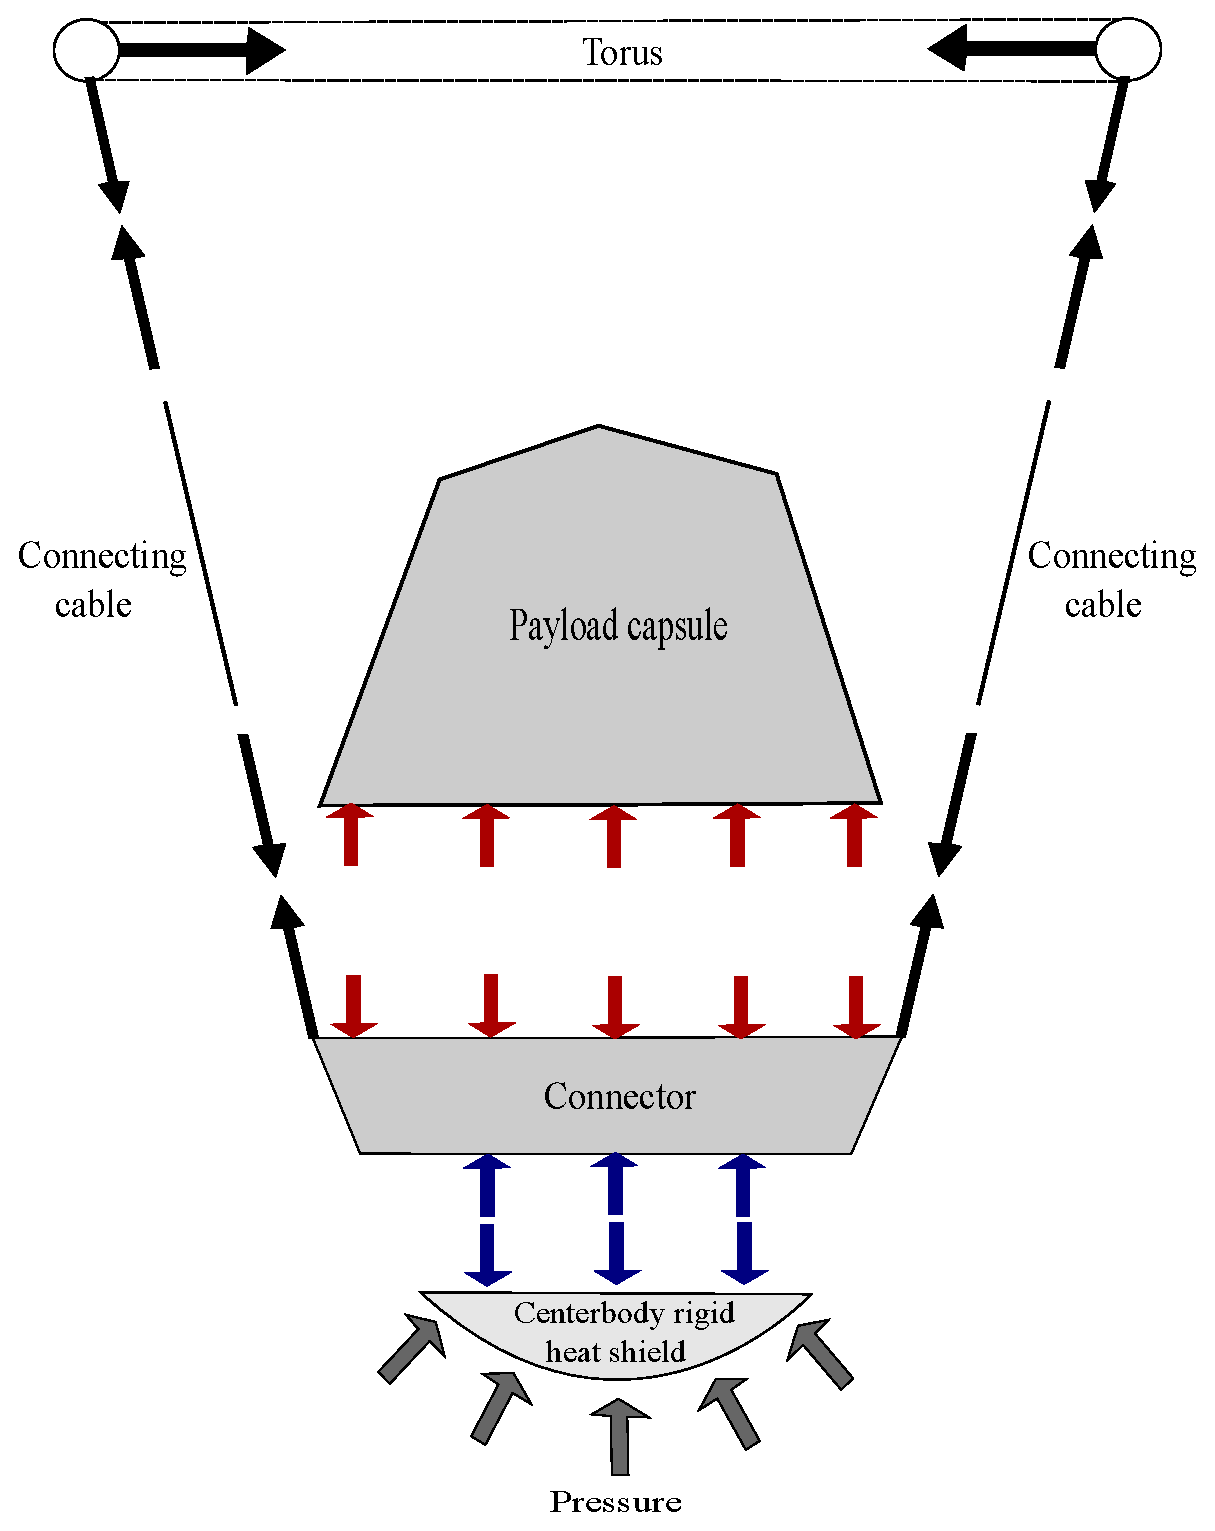
\includegraphics[width = 0.4\textwidth]{Figure/FBD_trailing.eps}
\caption{A \gls{fbd} of the trailing configuration}
\label{fig:fbd_trailing}
\end{figure}

The trailing concept is loaded similar to the tension cone concept, except that the torus is placed behind the payload and connected by cables. These cables are loaded in tension and their connection to the centerbody induces local load and stress concentrations.

\paragraph{Rigid}

The rigid configuration is the most typical configuration and is frequently used for re-entry in the Earth atmosphere such as in the Apollo, Soyuz and planned Orion mission. Figures \ref{fig:conc_rigid} and \ref{fig:fbd_rigid} show the rigid configuration. This design features a rigid heat shield in front of the payload and is the only concept featuring no inflatable parts.

\begin{figure}[H]
\centering

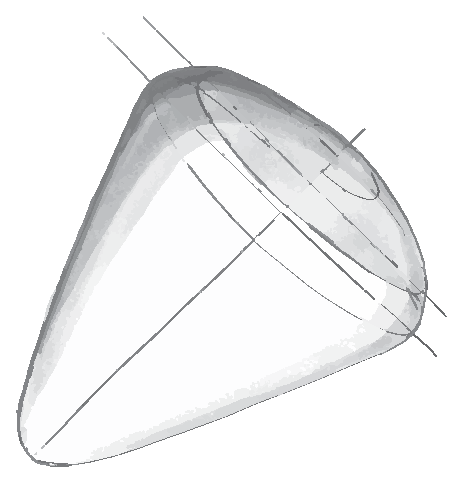
\includegraphics[angle=180, width = 0.3\textwidth]{Figure/rigid.eps}
\caption[An impression of a rigid configuration]{An impression of a rigid configuration\textsuperscript{\ref{fn:irene}}}

\label{fig:conc_rigid}
\end{figure}

\begin{figure}[H]
\centering
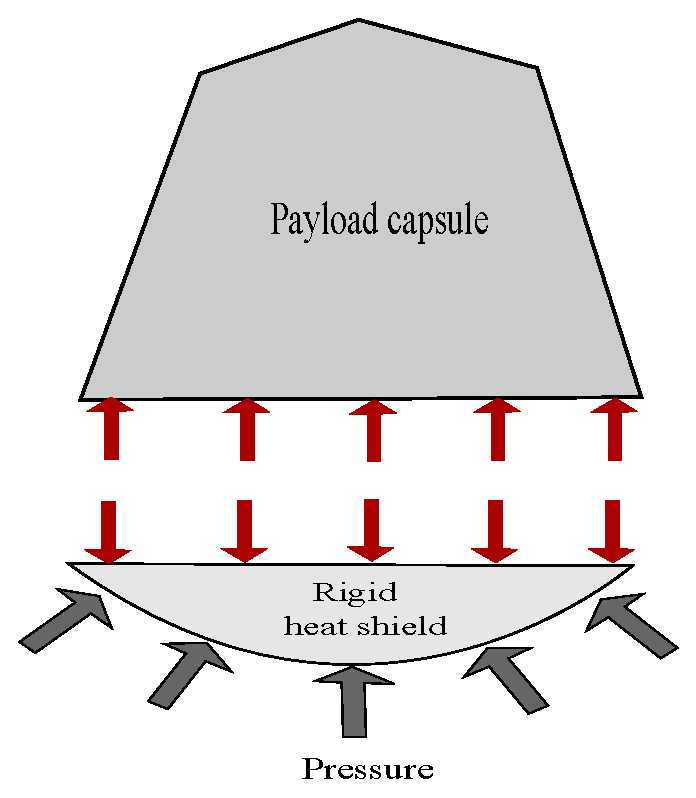
\includegraphics[width = 0.3\textwidth]{Figure/FBD_rigid.eps}
\caption{A \gls{fbd} of the rigid configuration}
\label{fig:fbd_rigid}
\end{figure}

\subsection{Concept control systems} \label{sec:ccs}
This section discusses the control systems of the \gls{dot} in Figure \ref{fig:dotcontrol}. This explains the concepts that were eliminated in Table \ref{tab:designconcepts}, denoting feasible and infeasible combinations respectively.

The control options are not yet further detailed within the Mid-Term Report, merely their feasibility and development risk for the concepts is checked. In the estimation of development risk and control system mass the feasible control concepts and the aerodynamic properties of the concepts are taken into account. The former is detailed here and in the risk estimations of Chapter \ref{ch:riskestimation}, the latter in Chapter \ref{ch:aero_analysis}.

\subsubsection{\gls{cg} offset}
A \acrfull{cg}-offset can be used in two ways: A static \gls{cg}-offset, which is typically used, and a actively controlled \gls{cg} offset system. The latter has already been demonstrated in the \gls{irve}-3 mission \cite{Dillman2012}. This was, however, considering smaller payload module mass fractions. Applying a \gls{cg} offset yields a change in the moment balance around the \gls{cg}. In a \gls{cg}-offset control system this property is actively used for the manipulation of the system. The use of a \gls{cg}-offset control system does however have speed limitations as changes in the location of the centre of gravity are slow.

An active \gls{cg}-offset system for the trailing and combined configurations was not deemed feasible due to the existence of aft elements which are connected to the capsule through a non-rigid connection such as a cable. Thus, for the trailing concept active \gls{cg}-offset control was not deemed feasible.

\subsubsection{Thrusters}
Thrusters are the only internal control system that was deemed feasible and will hence always be featured on the spacecraft since control outside the Martian atmosphere is required as well. Thrusters can however also be employed as a primary control system, which obviously increases the mass and usage of the systems.

Thrusters are deployed in pairs for the control of the spacecraft, such that they can deliver a torque couple. The amount of torque delivered is a linear function of the relative distance between the thrusters and is constrained for this design by launcher constraints. 

In terms of development risk thrusters are frequently used and feature minimal risk.

Thrusters are not considered for the trailing and combined configuration. Due to the aft elements of these designs thruster cannot be considered as the primary control mechanism. Due to the large moments of inertia (due to aft elements) and very high stability of the aft systems (e.g. compare to a parachute) thrusters cannot be considered due their inefficiency. 

\subsubsection{Control surfaces}
Active control surfaces have been subdivided into two forms; body flaps and morphing, both of which are covered below.

\paragraph{Body flaps}
A control system with body flaps features deployable surfaces to manipulate the flow around the spacecraft. Body flaps have previously been deployed at for example the Space Shuttle missions. It must however be noted that its usage was limited to supersonic Mach numbers at higher atmospheric densities. As such it is a possible control concept for the rigid structure.

Body flaps on inflatable structures have not yet been featured and are not deemed feasible. Since body flaps need to based inside the flow, positioning is not possible. In these designs the inflatable is the part placed within the flow. Do to the nature of deployment and the structural layout of these systems body flaps are not deemed to be feasible. The usage of body flaps for the Mach numbers considered would also incur a significant development risk.

\paragraph{Morphing}
In morphing concepts the whole external shape of the decelerator is changed to control the spacecraft. This is not possible for rigid structures as no morphable parts exist. 
 For the inflatable structures morphing is deemed possible with the exception of the isotensoid design and is already being investigated \cite{Hughes2011}. In the isotensoid design the whole outside is covered by inflatable. The whole inflatable can thus only be formed by usage of the gas inside. This is however not deemed possible due to the usage of ram-air as inflation mechanism.

Morphing of the trailing ballute configuration would be done via the payload-ballute connection much like for example a parachute.

In terms of development risk morphing of the structure is mostly at a very early conceptual phase posing significant development risks. Investigations for morphing of a stacked toroid configuration have for example been performed \cite{Green2013} but no actual testing is done.
